 
\noindent
Dieser Abschnitt legt die theoretischen Grundlagen von Operationsverstärkern dar.

\subsection{Charakteristiken}

\noindent 
Ein Operationsverstärker ist ein Differenzenverstärker, d.h., die Ausgangsspannung ist proportional zur Differenz der beiden Eingangsspannungen:
\begin{equation*}
    U_\text{A} = V \cdot \left( U_\text{P} - U_\text{N}\right)\, .
\end{equation*}
Die Ausgangsspannung ist phasengleich mit $U_\text{P}$, die am nicht-invertierenden Eingang ($+$) anliegt, und gegenphasig zu $U_\text{N}$, die am invertierenden Eingang ($-$) anliegt. Das Schaltbild eines Operativverstärkers ist in \autoref{fig:schaltung} dargestellt.

\begin{figure}%
    \centering%
    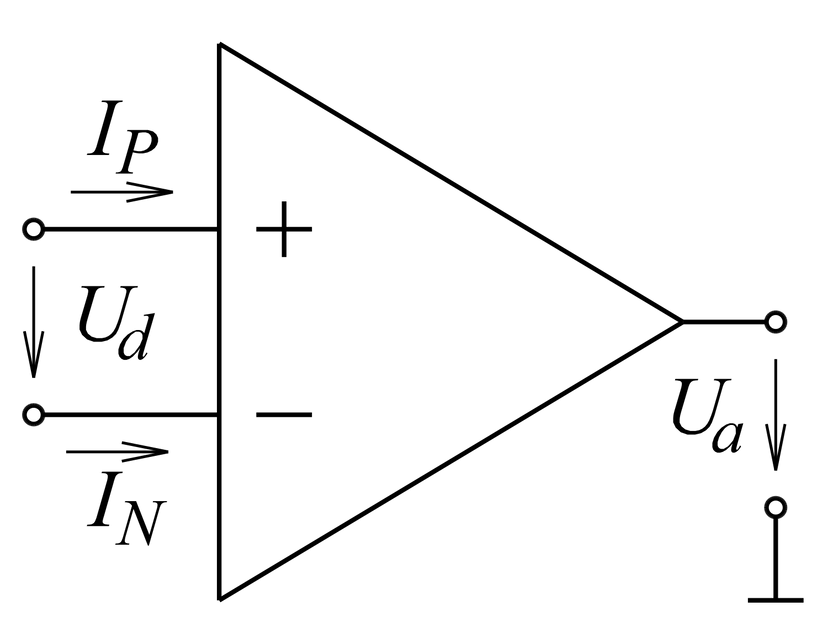
\includegraphics[width=0.8\textwidth]{Bilder/OpAmp.png}%
    \caption{Schaltbild eines Operationsverstärkers.\cite{OpAmp1}}%
    \label{fig:schaltung}%
\end{figure}%

Die Proportionalität der Ausgangsspannung zur Differenz der Eingangsspannungen gilt nur für:
\begin{equation*}
    - U_\text{S} < U_\text{A} < U_\text{S}\, ,
\end{equation*}
außerhalb dieses Bereichs ist die Ausgangsspannung $\pm U_\text{S}$. Dies ist in \autoref{fig:kennlinie} dargestellt.

\begin{figure}%
    \centering%
    
    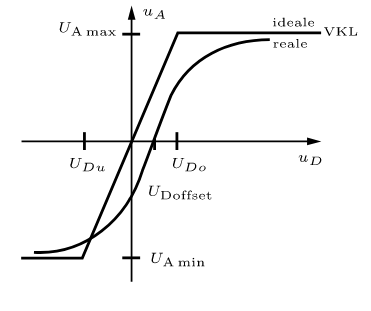
\includegraphics[width=0.4\textwidth]{Bilder/kennlinie_buch.png}%
    \caption{Kennlinie eines idealen und eines realen Operationsverstärkers. \cite{BrabetzHaasSpieker+2015}}%
    \label{fig:kennlinie}%
\end{figure}%

In \autoref{fig:kennlinie} ist zu sehen, dass die Ausgangsspannung $U_\text{A}$ linear mit der Eingangsspannungsdifferenz $U_\text{D}$ variiert, solange $- U_\text{S} < U_\text{A} < U_\text{S}$ gilt. Die Spannungsdifferenzen, bei denen diese Sättigung eintritt, werden als $U_\text{Du}$ und $U_\text{Do}$ bezeichnet.

Ein idealer Operationsverstärker hat eine unendliche Leerlaufverstärkung $V$, unendlich große Eingangswiderstände $r_\text{e,p}$ und $r_\text{e,n}$, um den Stromfluss im Verstärker zu verhindern, und einen Ausgangswiderstand $r_\text{A}$ von $0$. Die Übertragungsbandbreite reicht von $0$ bis $\infty$, und es tritt keine Phasenverschiebung auf.

Ein realer Operationsverstärker hingegen hat eine Leerlaufverstärkung von $V \propto 10^4$-$10^6$. Die Eingangswiderstände sind nicht unendlich groß, aber üblicherweise größer als $\SI{1}{\mega\ohm}$. Der Ausgangswiderstand liegt im Bereich von $\SI{10}{\ohm}$ - $\SI{1000}{\ohm}$. Die Übertragungsbandbreite hat eine obere Grenze, die sich im Bereich von $\SI{10}{\hertz}$ bis $\SI{10}{\kilo\hertz}$ befindet. Es tritt eine Phasenverschiebung auf.

Die Unterschiede zwischen einem realen und einem idealen Operationsverstärker führen zu geringfügigen Abweichungen, die kleine Korrekturen in den Berechnungen erfordern. Einige Phänomene, die daraus resultieren, werden im folgenden Abschnitt besprochen.

\noindent 
Wenn an beiden Eingängen die gleiche Spannung $U_\text{Gl}$ anliegt, sollte bei einem idealen Operationsverstärker eine Ausgangsspannung $U_\text{A} = \SI{0}{\volt}$ auftreten. Bei einem realen Verstärker misst man jedoch eine Ausgangsspannung $\increment U_\text{A}$.

Dieses Phänomen wird als Gleichtaktverstärkung bezeichnet und durch die Formel
\begin{equation}
    V_\text{Gl} = \frac{\increment U_\text{A}}{U_\text{Gl}}\, .
    \label{eqn:verstaerkung}
\end{equation}
parametrisiert. Zudem ist eine Offsetspannung zu messen, da eine Ausgangsspannung zu messen ist, falls beide Eingangsspannungen $0$ betragen. Die Offsetspannung $U_0$ ist als 
\begin{equation*}
    U_0 = U_\text{P} - U_\text{N}
\end{equation*}
definiert, wobei die Eingangsspannungen so gewählt sind, dass $U_\text{A}=0$ gilt.

Da bei einem realen Operationsverstärker endliche Eingangswiderstände auftreten, gibt es einen endlichen Eingangsruhestrom 
\begin{equation*}
    I_\text{B} = \frac{1}{2}\left( I_\text{P} + I_\text{N}\right)\, .
\end{equation*}
Analog dazu lässt sich ein Offsetstrom $I_0$ definieren, 
\begin{equation*}
    I_0 = I_\text{P} - I_\text{N}\quad \text{bei}\, U_\text{P} = U_\text{N}=0\, .
\end{equation*}
Abschließend sind die Differenzwiderstände
\begin{equation*}
    r_\text{P} = \begin{cases}
        \frac{\increment U_\text{P}}{\increment I_\text{P}} , & U_\text{N}=0\\
        \frac{\increment U_\text{N}}{\increment I_\text{N}} , & U_\text{P}=0
    \end{cases}\, ,
\end{equation*}
und der Gleichtakteingangswiderstand 
\begin{equation*}
    r_\text{Gl} = \frac{U_\text{Gl}}{I_\text{Gl}}
\end{equation*}
zu nennen.

Diese Phänomene erklären die leicht unterschiedliche Kennlinie in \autoref{fig:kennlinie}.

\subsection{Schaltbeispiele mit Operationsverstärkern}

\noindent 
In diesem Abschnitt werden die im Versuch verwendeten Schaltungen vorgestellt. 

\subsubsection{Invertierender Linearverstärker}

\noindent 
Da die Ausgangsspannung bei einem normalen realen Operationsverstärker schnell in den gesättigten Bereich übergeht, kann stattdessen ein invertierender Linearverstärker verwendet werden. Dazu wird die Ausgangsspannung über einen Widerstand $R_2$ an den invertierenden Eingang des Operationsverstärkers gegeben, wie in \autoref{fig:invertierter_lin} dargestellt. Dieses Verfahren wird auch als Gegenkopplung bezeichnet. Bei einer Zunahme der Ausgangsspannung kommt es zu einer Abnahme der Eingangsspannung. 

%\begin{figure}[H]%
%    \centering%
    %\includegraphics[width=0.4\textwidth]{images/invertierter_lin.png}%
%    \caption{Schaltbild eines gegengekoppelten invertierenden Linearverstärkers. \cite{V51}}%
%    \label{fig:invertierter_lin}%
%\end{figure}%

\noindent
Nach der Proportionalität der Ausgangsspannung zur Differenz der Eingangsspannungen gilt hier 
\begin{equation}
    U_\text{N} = - \frac{U_\text{A}}{V}\, .
\end{equation}
Für den Knotenpunkt vor dem invertierenden Eingang gilt bei $I_\text{N} = 0$ demnach 
\begin{equation*}
    \frac{U_\text{N} - U_1}{U_\text{A} - U_1} = \frac{R_1}{R_1 + R_\text{N}}\, .
\end{equation*}
Hieraus folgt für die Verstärkung $V'$: 
\begin{equation*}
    \frac{1}{V'} = - \frac{U_1}{U_\text{A}} = \frac{1}{V} + \frac{R_1}{R_\text{N}}\left(1 + \frac{1}{V}\right) \approx \frac{1}{V} + \frac{R_1}{R_\text{N}}\, ,
\end{equation*}
wobei die Näherung $V\gg 1$ genutzt wird. Es ist gut zu sehen, dass die Verstärkung bei $\frac{R_\text{N}}{R_1} \ll V$ quasi nur noch von dem Verhältnis der Widerstände abhängig ist. Da die Verstärkung $V$ stark schwanken kann, beispielsweise aufgrund der Temperatur, erhöht diese Gegenkopplung damit die Stabilität des Verstärkers. Mit dem Faktor 
\begin{equation*}
    g \coloneq \frac{V}{V'}
\end{equation*}
wird der Ausgangswiderstand verkleinert. Außerdem wird die Bandbreite um g erhöht, wie es in \autoref{fig:frequgang} zu sehen ist.
 
        


\begin{figure}[H]
    \centering
    %\includegraphics[width=0.6\textwidth]{images/frequenzgang_lin.png}
    \caption{Frequenzgang des Linearverstärkers. \cite{V51_old}}
    \label{fig:frequgang}
\end{figure}

\subsubsection{Umkehrintegrator}

\noindent
Ein Umkehrintegrator lässt sich wie in \autoref{fig:umkehrint} aufbauen. Im Unterschied zum invertierenden Linearverstärker ist hier ein Kondensator in der Rückkopplungsschleife eingebaut.

%\begin{figure}[H]
%    \centering
    %\includegraphics[width=0.4\textwidth]{images/Umkehrintegrator.png}
%    \caption{Schaltbild eines Umkehrintegrators. \cite{V51}}
%    \label{fig:umkehrint}
%\end{figure}

\noindent
Gemäß der Knotenregel ergibt sich für den Knotenpunkt vor dem invertierenden Eingang 
\begin{equation*}
    I_1 + I_\text{C} = 0\, ,
\end{equation*}
wobei hier bereits $I_\text{N} = 0$ gesetzt wurde, da die Spannung $U_\text{N}$ verschwindet. Es gilt 
\begin{align*}
    I_1 &= \frac{U_1}{R_1} \\ 
    \int I_\text{C} \, \text{d}t &= C U_\text{A}\, ,
\end{align*}
sodass sich die Ausgangsspannung zu 
\begin{equation*}
    U_\text{A} = - \frac{1}{RC} \int U_1 \, \text{d}t
\end{equation*}
berechnet. Die Ausgangsspannung ergibt sich also aus dem Integral der Eingangsspannung, was den Namen der Schaltung motiviert. Für eine Eingangsspannung $U_1 = U_0 \sin(\omega t)$ folgt somit eine Ausgangsspannung 
\begin{equation}
    U_\text{A} = \frac{U_0}{RC\omega} \cos(\omega t)\, .
    \label{eqn:int}
\end{equation}

\subsubsection{Invertierender Differenzierer}

\noindent
Ein invertierender Differenzierer ist in \autoref{fig:inverdiff} dargestellt. Es ist zu erkennen, dass sich zum Umkehrintegrator nur die Platzierung des Widerstandes und des Kondensators vertauscht hat.

%\begin{figure}[H]
%    \centering
    %\includegraphics[width=0.4\textwidth]{images/invertierter_diff.png}
%    \caption{Schaltbild eines invertierenden Differenzierers. \cite{V51}}
%    \label{fig:inverdiff}
%\end{figure}

\noindent
Die Knotenregel für den Knotenpunkt vor dem invertierenden Eingang ergibt hier 
\begin{equation*}
    I_1 + I_\text{A} = 0\, ,
\end{equation*}
wobei sich die einzelnen Ströme zu 
\begin{align*}
    I_1 &= \dot{Q} = C \cdot \dot{U_1} \\
    I_\text{A} &= \frac{U_\text{A}}{I_\text{A}}
\end{align*}
ergeben. Dadurch steht die Ausgangsspannung in einem Zusammenhang mit der zeitlichen Ableitung der Eingangsspannung
\begin{equation*}
    U_\text{A} = - RC \cdot \dot{U_1}\, .
\end{equation*}
Für eine sinusförmige Eingangsspannung $U_1 = U_0 \sin(\omega t)$ ergibt sich dann eine Ausgangsspannung 
\begin{equation}
    U_\text{A} = - R C U_0 \omega \cdot \cos(\omega t)\, ,
    \label{eqn:dif}
\end{equation}
die eine lineare Proportionalität zur Frequenz aufweist.

\subsubsection{Nichtinvertierender Schmitt-Trigger}

\noindent 
Bei dieser Schaltung wird die Ausgangsspannung über einen Widerstand an den nichtinvertierenden Eingang des Operationsverstärkers gegeben. Dies ist in \autoref{fig:schmitttrig} dargestellt.

%\begin{figure}[H]
%    \centering
    %\includegraphics[width=0.4\textwidth]{images/schmitt_trigger.png}
%    \caption{Schaltbild einer Schmitt-Triggerschaltung. \cite{V51}}
%    \label{fig:schmitttrig}
%\end{figure}
\noindent
Es kommt somit zu einer Mitkopplung, bei der ein größeres Ausgangssignal ein größeres Eingangssignal erzeugt. Dies führt zu einem recht instabilen Verhalten, und die Ausgangsspannung springt abrupt auf $\pm U_\text{S}$, sobald die Eingangsspannung bestimmte Schwellenwerte erreicht.% Dies ist in \autoref{fig:abbschmitt} dargestellt. Das Ausgangssignal ist also eine Rechteckspannung.

%\begin{figure}[H]
%    \centering
    %\includegraphics[width=0.4\textwidth]{images/schmitt_trig_dia.png}
%    \caption{Ein $U_E$-$U_\text{A}$ Diagramm des Schmitt-Triggers. \cite{Joachim}}
%    \label{fig:abbschmitt}
%\end{figure}

Die Schwellwerte der Eingangsspannung sind 
\begin{align*}
    - \frac{R_1}{R_\text{P}} U_\text{S} && \text{und} && \frac{R_1}{R_\text{P}} U_\text{S} \, .
\end{align*}

\subsubsection{Signalgenerator}

\noindent 
Wenn ein Schmitt-Trigger an einen Umkehrintegrator angeschlossen wird, wie in \autoref{fig:signal} dargestellt, beginnt das System spontan zu schwingen. 

%\begin{figure}[H]
%    \centering
    %\includegraphics[width=0.8\textwidth]{images/signalgenerator.png}
%    \caption{Schaltbild eines Signalgenerators. \cite{V51}}
%    \label{fig:signal}
%\end{figure}

\noindent
Die konstante Spannung, die vom Schmitt-Trigger ausgeht, wird integriert. Die Ausgangsspannung aus dem Umkehrintegrator wird als $U_1$ verwendet, sodass die Eingangsspannung des Schmitt-Triggers einen Schwellenwert erreicht. In den Integrator wird eine konstante Spannung mit entgegengesetztem Vorzeichen eingespeist. Insgesamt ergibt sich als Ausgangsspannung eine Dreiecksspannung mit 
\begin{align*}
    \text{Frequenz}\, : & & \text{und} & & \text{Amplitude}\, :& \\
    \nu_\text{Dreieck} &= \frac{R_2}{4 C R_1 R_3} & & &A &=  U_\text{max} \frac{R_1}{R_2} \, .
\end{align*}

\subsubsection{Generator mit variierender Amplitude}
Ein Generator mit variierender Amplitude besteht aus zwei Integratoren und einem Invertierer. Dadurch kann eine gedämpfte Oszillation hergestellt 
werden. Der Aufbau ist in \autoref{fig:generatorvar} dargestellt.
\begin{figure}
    \centering
    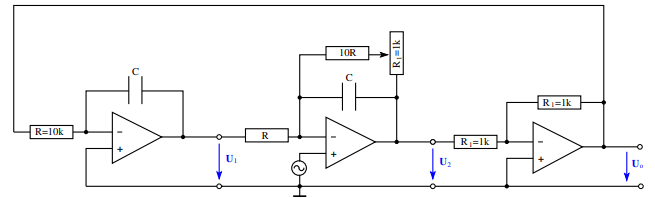
\includegraphics[width=0.8\textwidth]{generatorvar.png}
    \caption{Schaltbild eines Generators mit variierenden Amplituden \cite{ap51}.}
    \label{fig:generatorvar}
\end{figure}
Die gedämpfte Oszillation lässt sich über die Differentialgleichung
\begin{equation*}
    \frac{\symup{d^2}U_A}{\symup{d}t^2}- \frac{\eta}{10RC}\frac{\symup{d}U_A}{\symup{d}t}+\frac{1}{R^2C^2}U_A = 0
\end{equation*}
beschreiben. Dabei ist $\eta$ die Dämpfungskonstante. 
Obige Gleichung ist lösbar mit 
\begin{equation}
    U_A(t) = U_0\cdot exp\lvert \frac{t}{\tau}\rvert \cdot sin \lvert 2\pi\frac{t}{T}\rvert \,\,\text{.}
    \label{eqn:dgllsg}
\end{equation}
Hierbei ist $\tau = \frac{20RC}{\eta}$ die Abklingdauer und $T=2\pi RC$ die Schwingungsdauer.